% Copyright Ben Paul Wise. All Rights Reserved.
% The maneuver studies as a standalone document.  The text is shared with the design memorandum
% (circling_dragons_map_and_rules_V3.tex) through sections/sheet-75km.tex and sections/maneuver-studies.tex.
\documentclass[11pt]{article}
\usepackage[letterpaper,margin=.85in]{geometry}
\usepackage[T1]{fontenc}\usepackage{lmodern}\usepackage{microtype}
\usepackage{booktabs,enumitem,graphicx,float}
\usepackage[hidelinks,bookmarksnumbered,bookmarksopen]{hyperref}
\usepackage{tikz}
% Copyright Ben Paul Wise. All Rights Reserved.
% The full-page locator map before each section of figures: the standard sheet with the area of the section's
% figures boxed in black.  Shared by circling_dragons_map_and_rules_V3.tex and maneuver_studies_75km.tex; needs
% graphicx and tikz.  The boxes are generated by map_graphics/xml/tools/cd/illustrate.py (locator-boxes.tex).
% The map is set once in a box, so the PDF carries one copy of the image however many locators there are.
% Copyright Ben Paul Wise. All Rights Reserved.
% Generated by map_graphics/xml/tools/cd/illustrate.py; do not edit.  The area each section's figures show
% on the standard sheet, as a TikZ rectangle in fractions of the sheet (x from the left, y from the bottom).
\def\cdboxIchigo{(0.1568,0.0943) rectangle (0.5986,0.6013)}   % 1-ichigo-setup
\def\cdboxReflux{(0.1568,0.0943) rectangle (0.5986,0.6013)}   % 2-reflux-setup
\def\cdboxAugust{(0.3402,0.5942) rectangle (0.9654,0.9891)}   % 3-august-setup
\def\cdboxRace{(0.2587,0.4484) rectangle (0.8432,0.9241)}   % 4-race-setup
\def\cdboxChangsha{(0.3198,0.2297) rectangle (0.4968,0.3746)}   % a1-changsha-position
\def\cdboxHengyang{(0.2995,0.1568) rectangle (0.4764,0.3225)}   % b1-hengyang-position
% Copyright Ben Paul Wise. All Rights Reserved.

\newsavebox{\cdmapbox}
\AtBeginDocument{\sbox{\cdmapbox}{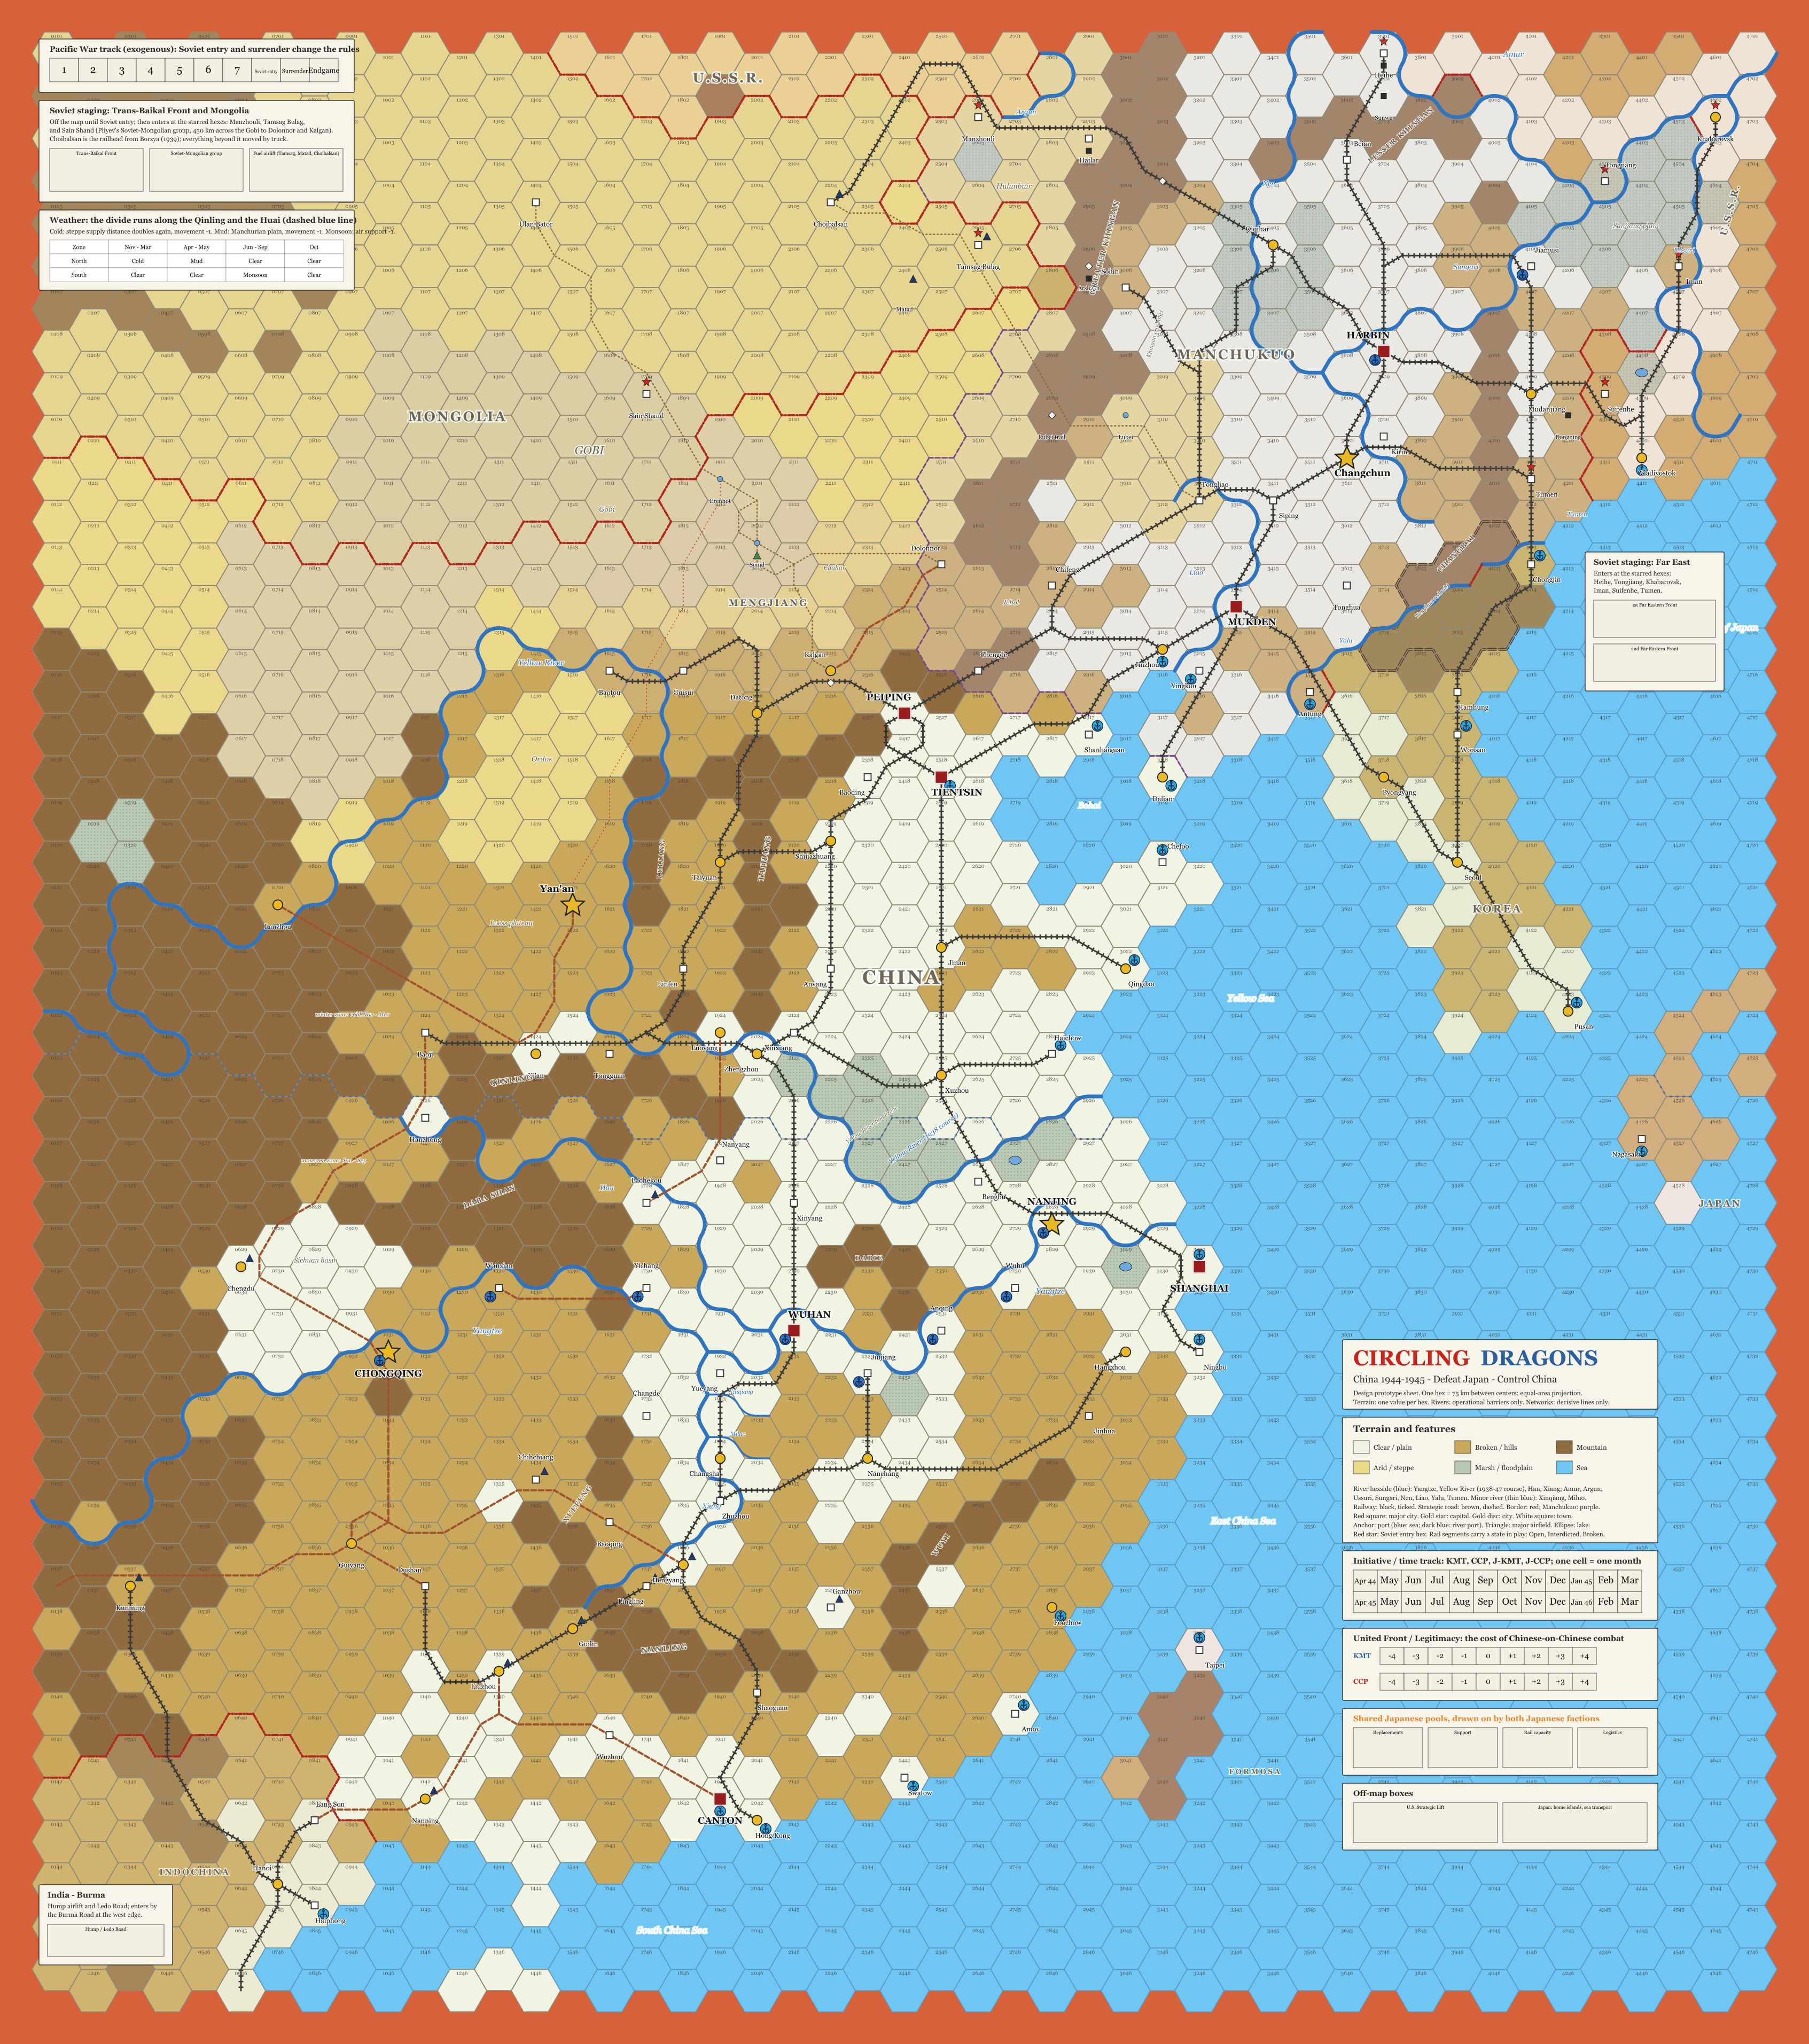
\includegraphics[width=\textwidth,height=.84\textheight,keepaspectratio]{../map_graphics/xml/circling-dragons.png}}}
\newcommand{\locator}[2]{%
  \clearpage
  \begin{figure}[p]\centering
  \begin{tikzpicture}
    \node[anchor=south west,inner sep=0] (map) at (0,0) {\usebox{\cdmapbox}};
    \begin{scope}[x={(map.south east)},y={(map.north west)}]
      \draw[white,line width=5pt] #1;
      \draw[black,line width=2.6pt] #1;
    \end{scope}
  \end{tikzpicture}
  \caption{#2}
  \end{figure}
  \clearpage}
% Copyright Ben Paul Wise. All Rights Reserved.

\setlist{nosep}
\title{\textbf{Circling Dragons}\\\large Two Maneuver Studies on the 75 km Sheet\\\normalsize China, 1941--1944}
\author{}\date{Draft study --- October 2026}
\newcommand{\illus}[2]{\begin{figure}[p]\centering\includegraphics[width=\textwidth,height=.82\textheight,keepaspectratio]{illustrations/#1.png}\caption{#2}\end{figure}}
\begin{document}\maketitle

\begin{abstract}
The standard \emph{Circling Dragons} sheet has had 75 km between hex centres since October 2026; the first sheet had 100 km. At 100 km the Hunan corridor is too narrow for two maneuvers that decided its battles: Xue Yue's defence of Changsha in 1939--42, and the Japanese envelopment of Hengyang in 1944. This study describes the 75 km sheet and works both maneuvers through on it with the preliminary counter set, in nine figures, with the rules the figures assume. The same text is part of the design memorandum. The counts, values and rules are placeholders for the prototype.
\end{abstract}

\section{The standard sheet at 75 km}\label{sub:sheet75}
% Copyright Ben Paul Wise. All Rights Reserved.
% The standard sheet at 75 km: shared by circling_dragons_map_and_rules_V3.tex and maneuver_studies_75km.tex,
% each of which gives the heading.  Needs the labels sec:maneuvers and sub:mrules (maneuver-studies.tex).
The standard sheet has 75 km between hex centers. It replaced the first sheet, at 100 km, in October 2026, because at 100 km the Hunan corridor is too narrow for two maneuvers that decided its battles: Xue Yue's defense of Changsha in 1939--42 and the Japanese envelopment of Hengyang in 1944 (section~\ref{sec:maneuvers}).

Both sheets cover the same area and are built by the same programs from the same sources, so the scale is a setting of the build and the first sheet can still be produced for comparison. Every ruling made on the 100 km sheet was carried over: the named mountain ranges, the lakes and the Tonghua redoubt are lists of 100 km hexes, and each 75 km hex whose center falls in a listed hex takes the ruling. Three coastal hexes, each just under half land, were ruled land so that the railways of the Liaodong peninsula, the south shore of Hangzhou Bay and the Korean west coast stay on land. At Yueyang the Yangtze was moved to the north side of the city's hex, so that the railway south to Changsha does not cross it. Between Tongguan and Zhengzhou the Yellow River was moved to the north side of the Sanmenxia and Luoyang hexes, so that the Longhai railway stays on the south bank and crosses the river only on its 1938--47 course east of Zhengzhou. The Ussuri was extended two hexsides to join the Amur at Khabarovsk. The sheet passes the same validation and network checks as the first one.

\begin{center}
\begin{tabular}{lrr}
\toprule & First sheet & Standard sheet \\\midrule
Distance between hex centers & 100 km & 75 km \\
Columns by rows & 35 by 34 & 47 by 46 \\
Hexes on the sheet & 1,190 & 2,162 \\
Hexes in play (China, Manchukuo, Korea) & 672 & 1,187 \\
Mongolian hexes, open to Soviet formations only & 131 & 242 \\
Clear hexes across the corridor at Changsha & 2 & 3 \\
Clear hexes across the corridor at Hengyang & 2 & 3 \\
Hexes from Yueyang to Changsha & 1 & 2 \\
Hexes from Hankow to Dushan along the corridor & 12 & 15 \\
Sheet size with 3/4 inch hexes & 24 by 27 in & 32 by 36 in \\
\bottomrule
\end{tabular}
\end{center}

Of the hexes in play, the two sheets have nearly the same terrain: clear 26 and 27 percent, broken 33 and 32, mountain 24 and 23, steppe 15 and 15, marsh 3 and 3. The smaller hex does not make the country look flatter, so the terrain thresholds were left unchanged.

The standard sheet adds one line class, the \textbf{minor river}, drawn thinner than the major rivers and printed only where a minor river shaped a campaign. Two are printed: the Xinqiang and the Miluo, the delay lines north of Changsha on which Xue Yue's screens stood. Each crosses the railway column and the lane east of it, and each runs into the Xiang. The Laodao, the third of his lines, lies inside the Changsha hex and is not printed. In the provisional rules a minor river costs less to cross than a major river, and a formation behind one may withdraw before combat (section~\ref{sub:mrules}).

At 3/4 inch hexes the sheet is about 32 by 36 inches and fits on two 22 by 34 inch map sheets joined along their long edges. To keep the density of pieces of the first estimate, the counter set was grown to 126 unit pieces and 250 counters in all.

\begin{figure}[p]\centering
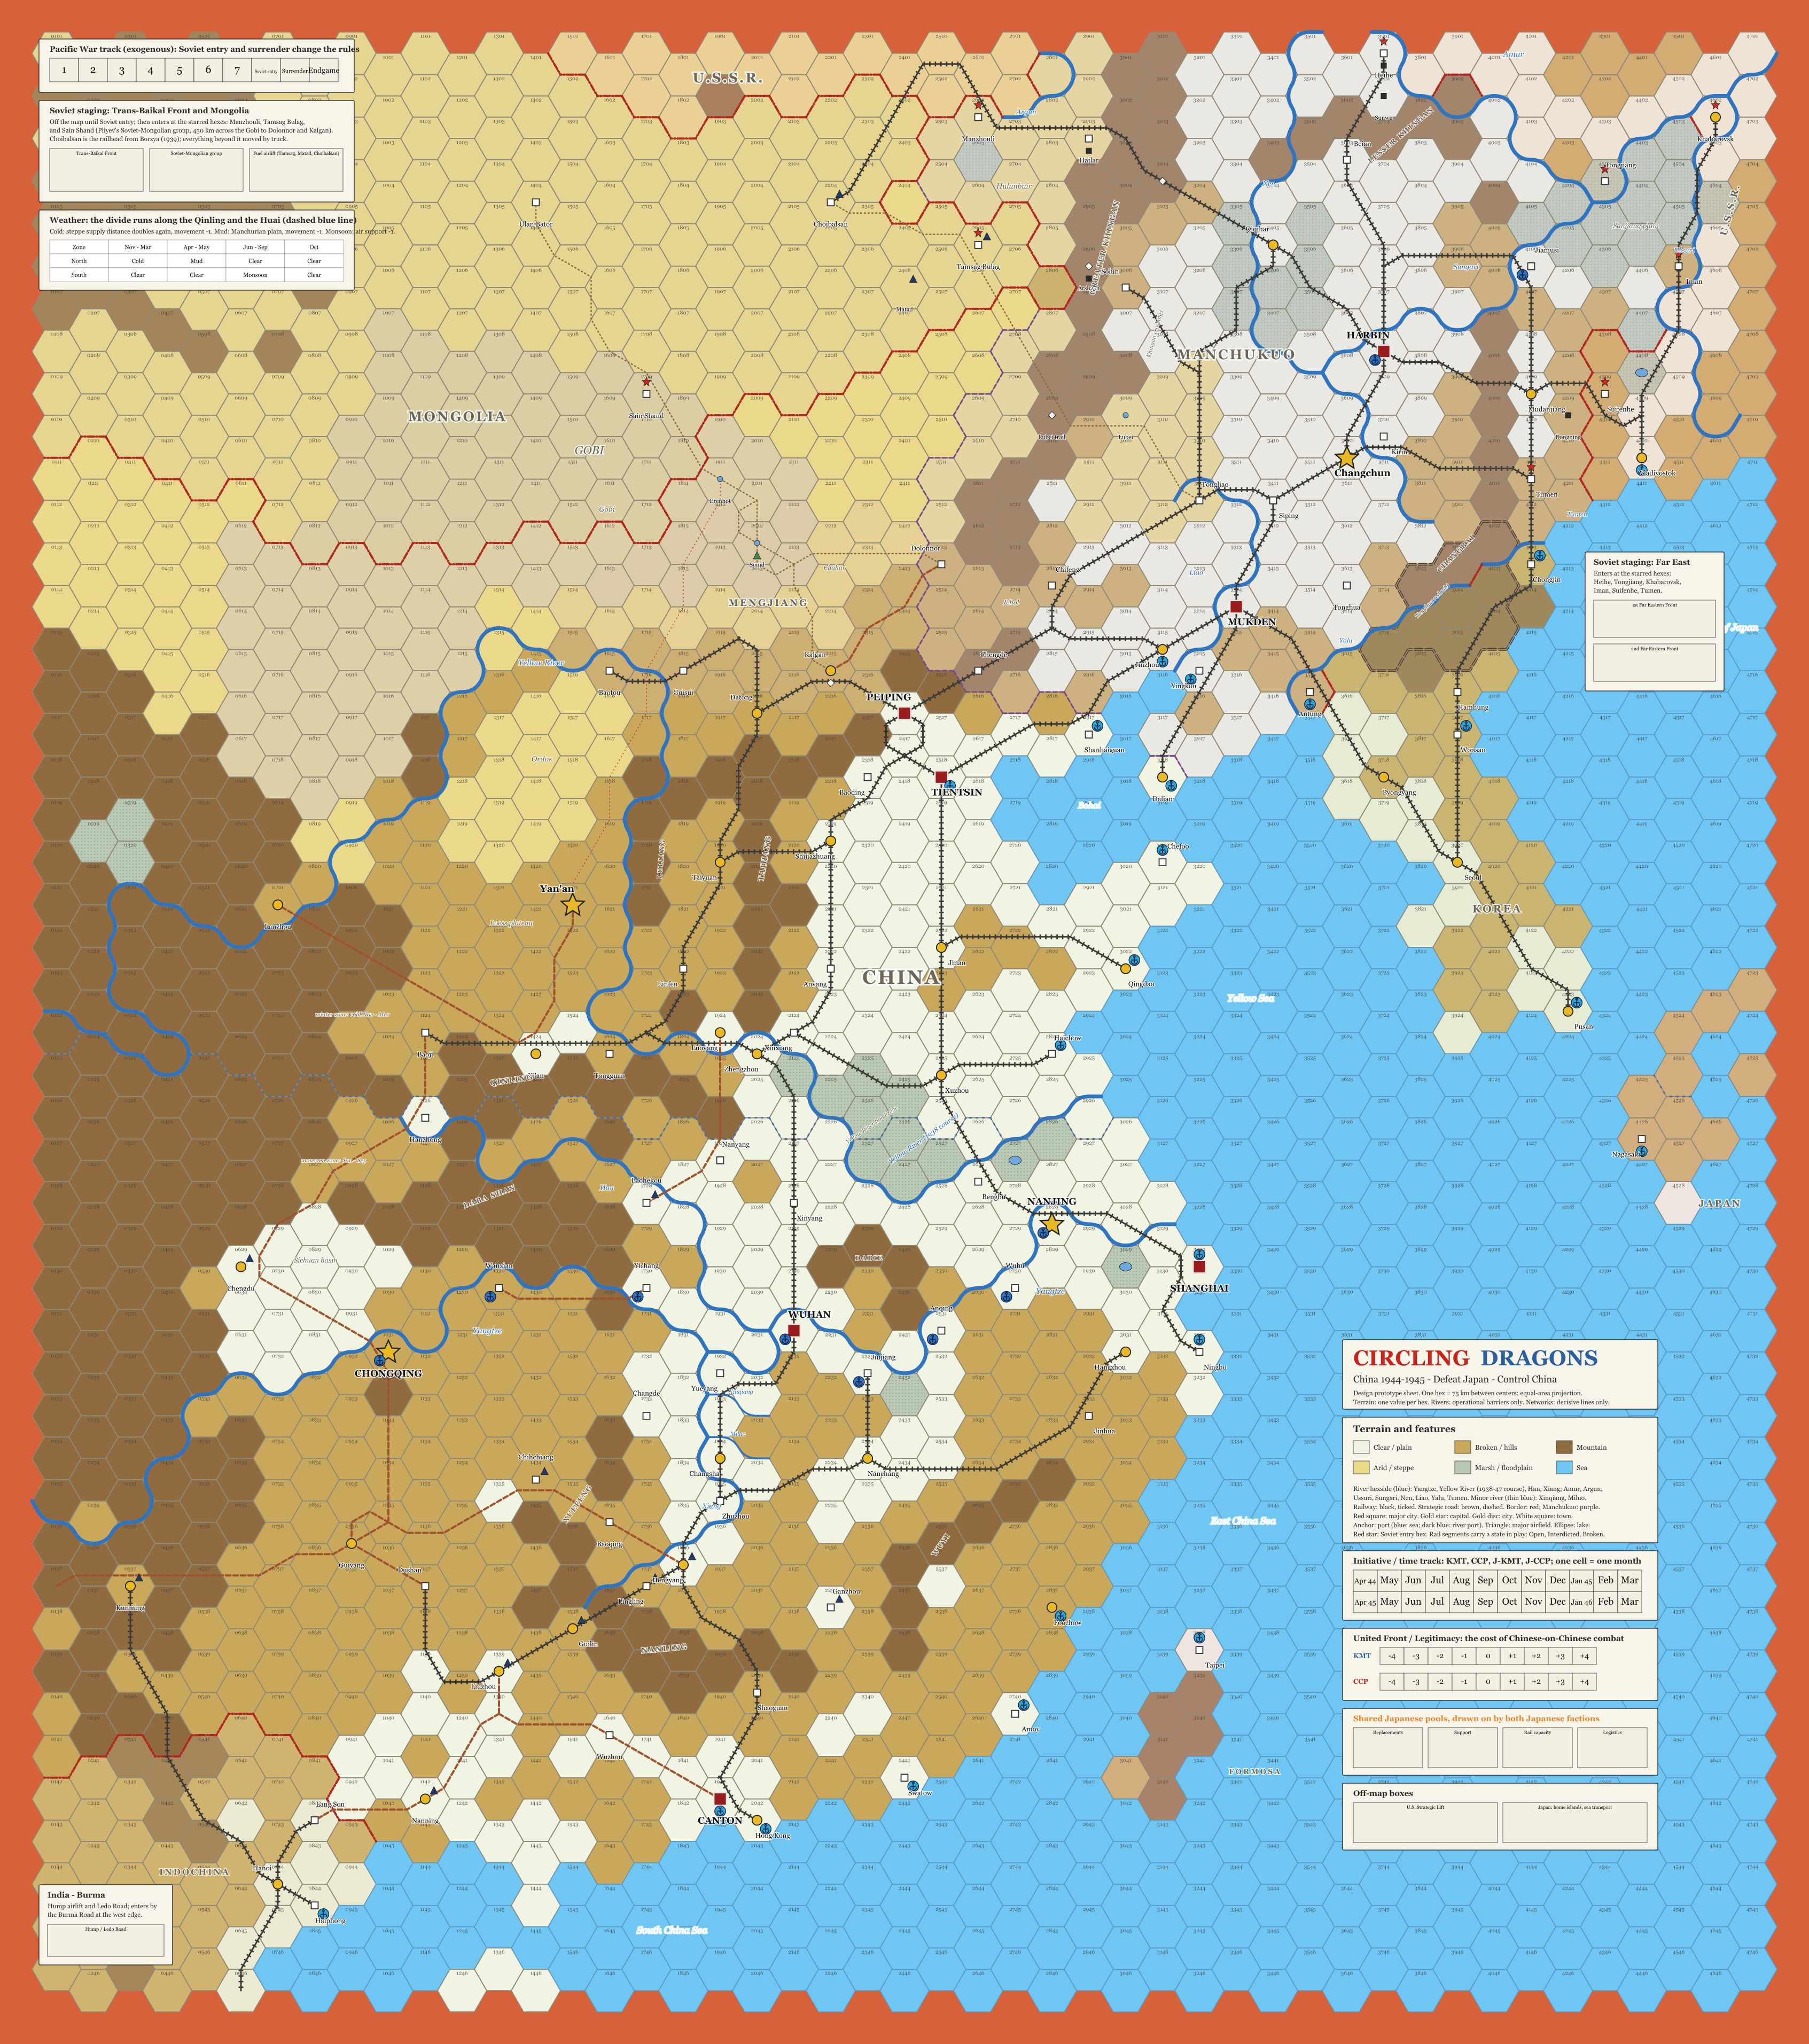
\includegraphics[width=\textwidth,height=.86\textheight,keepaspectratio]{../map_graphics/xml/circling-dragons.png}
\caption{The standard sheet, 75 km between hex centers. The furniture panels keep their size and their places in the corners where little fighting took place; the Mongolian features and the political layer are those of the first sheet.}
\end{figure}
% Copyright Ben Paul Wise. All Rights Reserved.


\section{The maneuver studies}\label{sec:maneuvers}
% Copyright Ben Paul Wise. All Rights Reserved.
% The two maneuver studies on the standard (75 km) sheet: shared by circling_dragons_map_and_rules_V3.tex and
% maneuver_studies_75km.tex, each of which gives the section heading (label sec:maneuvers) and defines \illus
% and \locator (sections/locator.tex).
% The figures are drawn by map_graphics/xml/tools/cd/illustrate.py from the tables in maneuvers.py.
The 75 km sheet was adopted because of two maneuvers the 100 km sheet had no room for: Xue Yue's defense of Changsha in 1939--42, and the Japanese envelopment of Hengyang in 1944. Both are shown here with the preliminary counter set, in nine figures drawn on crops of the standard sheet.

In these figures Japanese movement is dark red and KMT movement dark blue; a dashed line is a withdrawal, a green dashed line air supply. A yellow burst on a hexside is an attack across it. The numbered discs give the order of the moves within the figure. A piece shown with fewer step dots and a lower value has lost a step. The letters X and M mark the Xinqiang and the Miluo, the two minor rivers north of Changsha. The group-army pieces of the counter set stand in for the armies named in the text, and the positions are worked examples, not a scenario.


\clearpage
\locator{\cdboxChangsha}{Xue Yue's defense of Changsha: the area of the next five figures, boxed on the standard sheet, from Changde to Nanchang and from Wuhan to Zhuzhou.}
\subsection{Xue Yue's defense of Changsha}
\paragraph{Frame.} The Japanese 11th Army attacked Changsha from Yueyang three times, in September 1939, in September 1941, and from December 1941 to January 1942. Each time Xue Yue, commanding the 9th War Area, met the attack in the same way. Screening forces held the river lines north of the city (the Xinqiang, the Miluo and the Laodao) long enough to slow the advance, then gave way to the flanks rather than falling back on the city. The main body waited in the hills east of the railway, out of the attacker's reach, with a second group west of the Xiang. A strong garrison held Changsha itself. When the attacker reached the city, overextended and with his wings spread, the flank groups came out of the hills and closed in behind him. Xue Yue called this method ``heaven's furnace'' tactics. The Japanese withdrew from the third battle having lost heavily.
\paragraph{Why the smaller hex is needed.} At 100 km Yueyang and Changsha are adjacent, and the column of hexes east of the railway is both the attacker's flank lane and the defender's hill country. At 75 km there are two hexes from Yueyang to Changsha, with the Xinqiang and the Miluo across them, and east of the railway a lane of clear and broken hexes lies between the axis and the hills. The defender then has somewhere to step aside to, and the attacker's wing has a lane whose supply can be cut behind it.
\paragraph{In 1944.} The method failed in May and June 1944. The 11th Army came with eight divisions instead of four, on three columns: one down the railway, one through the eastern hills, and one down the west bank of the Xiang. The eastern column attacked the flank groups where they waited, the western column took Yuelu Shan across the river from the city, and Changsha fell on 18 June. The last figure of the study shows why: when the attacker is strong enough to fill the lanes as well as the axis, there is no lane left behind him to close.

\illus{a1-changsha-position}{Changsha 1941--42, the position. The 11th Army at the Yueyang railhead with air support, and a wing east of the railway. The screens stand behind the Xinqiang in the two hexes north of the city, with the Miluo at their backs; the garrison holds the fortified city, a west group stands across the Xiang, and the main body with the 9th War Area headquarters waits in the hills east of the railway.}
\illus{a2-changsha-advance}{Changsha, the advance. (1) The Japanese center crosses the Xinqiang. (2) The screen in its path withdraws west across the Xiang to the west group instead of falling back on the city. (3) The east wing crosses the Xinqiang and the Miluo into the lane and swings around toward the city from the east. (4) The screen in the lane withdraws into the hills, where the main body waits.}
\illus{a3-changsha-furnace}{Changsha, the flank groups strike. (1) The Japanese center attacks the city across the Miluo and is repulsed. (2) A KMT piece comes out of the hills into the lane behind the east wing. (3) The main body attacks the east wing from the hills. (4) The west group attacks the center from across the Xiang. The east wing is now out of supply, because every path back to Yueyang runs through a hex held by the KMT or in its zone of control, and the center is attacked from three sides.}
\illus{a4-changsha-withdrawal}{Changsha, the withdrawal. (1) The east wing breaks out through the lane, back over the Miluo and the Xinqiang, losing a step. (2) The KMT piece in the lane gives way and returns to the hills. (3) The center withdraws over the Xinqiang to Yueyang, also losing a step. (4) The west group follows into the hex north of the city and the screens are restored. The position is as it was before the attack, and the attacker is two steps weaker.}
\illus{a5-changsha-1944}{Changsha 1944, three columns. (1) The center attacks the city across the Miluo, and the city falls on 18 June. (2) The eastern column drives into the hills where the main body waited. (3) A second division enters the other hill hex. (4) The western column comes down the west bank of the Xiang to the far side of the city. The KMT flank groups are driven out of the hills and the west bank, each losing a step. Nothing remains to close in behind the center.}
\clearpage


\clearpage
\locator{\cdboxHengyang}{The envelopment of Hengyang: the area of the next four figures, boxed on the standard sheet, from Baoqing to Ganzhou and from Changsha to Guilin.}
\subsection{The envelopment of Hengyang}
\paragraph{Frame.} After Changsha the 11th Army moved on Hengyang, the junction of the Canton--Hankow and Hunan--Guangxi railways and the site of a Fourteenth Air Force field. The 68th and 116th Divisions reached the city on 23 June 1944, coming down both banks of the Xiang, while other divisions cut the railway to the south at Leiyang and screened the roads by which relief could come. Inside were the 10th Army under Fang Xianjue. The general assaults of 28 June and 11 July were repulsed with heavy loss. Relief columns, among them the 79th Army from the west and the 62nd Army from Guangxi in the southwest, tried to break the ring and were held off; the 62nd came within a few miles of the city. The Japanese brought up the 58th Division for a third assault on 4 August, and the 10th Army surrendered on 8 August, after 47 days.
\paragraph{Why the smaller hex is needed.} An envelopment needs the six hexes around the city to be occupied or held in a zone of control, and room outside the ring for the screens that keep the relief away. At 100 km Hengyang sits in a belt of two clear hexes between the Xuefeng and the hills to the east, and the ring hexes are the same hexes the relief must cross. At 75 km the belt is three clear hexes wide, the ring is a distinct band of six hexes, and the screens stand one hex further out.
\paragraph{The cost of the siege.} For the game, the important feature of the siege is its length, 47 days. The fortified-city rule should make the siege cost the Japanese two or three activations of five divisions, during which the KMT and the CCP act elsewhere on the time track and the shared Japanese pools are drawn down.

\illus{b1-hengyang-position}{Hengyang 1944, the position on 22 June. The 11th Army has taken Changsha: two divisions on the west bank, one on the east bank at Zhuzhou, two more to the east, and two at Changsha with air support. The 10th Army holds Hengyang, a fortified city with the Fourteenth Air Force. Relief groups stand at Baoqing in the west, in Guangxi in the southwest, and to the east.}
\illus{b2-hengyang-ring}{Hengyang, the ring closes, 23 June to 2 July. (1) The 116th Division comes down the west bank to the northwest of the city, across the road from Baoqing. (2) The 68th Division takes the hex northeast of the city. (3) The 13th Division swings around the east side to the southeast of the city and cuts the railway at Leiyang. (4) The 3rd Division blocks the east. (5) The 40th Division screens the west against the relief from Baoqing. The 58th Division comes up from Changsha as the reserve. The six hexes around the city are occupied or in a Japanese zone of control, and the city is out of supply.}
\illus{b3-hengyang-siege}{Hengyang, siege and relief in July. (1, 2) The assaults from the northeast and the northwest are repulsed, and the garrison loses a step. (3) The western relief attacks the 40th Division and is blocked. (4) The southwestern relief comes up to the ring. (5) The 116th Division attacks it, and (6) it falls back. (7) The eastern relief attacks the 3rd Division and is blocked. Air drops from the south are the city's only supply.}
\illus{b4-hengyang-fall}{Hengyang, the fall, 4 to 8 August. (1) The 58th Division comes up to the hex north of the city. (2) The 58th and 13th Divisions attack from the north and the southeast. (3) The 116th and 68th Divisions enter the city, each having lost a step in the siege. The 10th Army surrenders after 47 days. The next objectives are Lingling and Guilin.}
\clearpage

\subsection{Rules the maneuvers assume}\label{sub:mrules}
The figures assume the following rules. All are provisional, and the prototype will test them.
\begin{enumerate}
\item \textbf{Zones of control.} A formation's zone of control covers the six hexes around it, except across a major river or into a mountain hex. A supply path may not enter a hex in an enemy zone of control unless a friendly formation occupies it. This is what cuts the east wing at Changsha and closes the ring at Hengyang.
\item \textbf{Minor rivers.} A minor river hexside costs one extra movement point to cross, less than a major river, and does not block zones of control.
\item \textbf{Withdrawal before combat.} A formation in broken or mountain terrain, or behind a minor river, may withdraw one hex when an enemy formation moves adjacent, at the cost of one initiative space. This lets the screens step aside instead of standing to be destroyed.
\item \textbf{Fortified cities.} Attacks on a fortified city are halved, and the defender may convert one step loss into a retreat refused. The marker is removed when the city falls.
\item \textbf{Air supply.} A fortified city within range of a friendly air-support piece is in limited supply even when surrounded: it does not lose steps for lack of supply, but it may not attack.
\item \textbf{Out of supply.} A formation out of supply attacks at half strength and loses a step if it is still out of supply at the end of its next activation.
\item \textbf{Stacking.} Two unit pieces may stand in a hex, together with any number of markers and one air-support piece.
\end{enumerate}

\subsection{What the smaller hex provides}
\begin{enumerate}
\item At 75 km both maneuvers can be shown with the pieces of the preliminary set and a handful of ordinary rules. At 100 km neither could be shown without special rules, because the lanes and the ring merged with the axis.
\item The smaller hex does not by itself solve the tempo problem of Ichi-Go. The fifteen hexes from Hankow to Dushan still need the time track, the fortified-city rule and rail supply to take seven months.
\item The cost is 1,187 hexes in play instead of 672, two map sheets at 3/4 inch hexes, and 126 unit pieces instead of 72.
\item With the 75 km sheet the defender's maneuver in the Hunan corridor is part of the game, beside the time track and the crossed control.
\end{enumerate}
% Copyright Ben Paul Wise. All Rights Reserved.

\end{document}
% Copyright Ben Paul Wise. All Rights Reserved.
